\documentclass[tikz,border=6pt]{standalone}
\usepackage{amsmath,amssymb}
\usetikzlibrary{arrows.meta,patterns}
\begin{document}
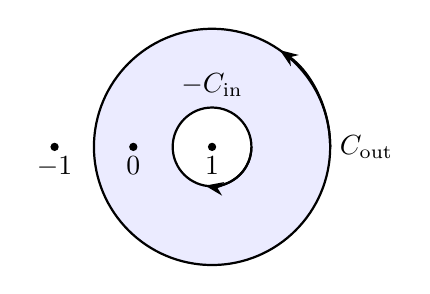
\begin{tikzpicture}[>=Stealth,scale=1]
 \fill[blue!8,even odd rule] (1,0) circle (1.5) (1,0) circle (.5);
 \draw[thick] (1,0) circle (1.5);
 \draw[->,thick] (2.5,0) arc (0:55:1.5);
 \draw[thick] (1,0) circle (.5);
 \draw[->,thick] (1.5,0) arc (0:-100:.5);
 \fill (0,0) circle (1.5pt) node[below]{$0$};
 \fill (1,0) circle (1.5pt) node[below]{$1$};
 \fill (-1,0) circle (1.5pt) node[below]{$-1$};
 \node[right] at (2.5,0) {$C_{\mathrm{out}}$};
 \node[above] at (1,.52) {$-C_{\mathrm{in}}$};
\end{tikzpicture}
\end{document}
